\documentclass[a4paper,11pt]{article}
\usepackage{amsmath,amsthm,amssymb}
\usepackage[utf8]{inputenc}
\usepackage[english,russian]{babel}
\usepackage[export]{adjustbox}
\usepackage{graphicx}
\usepackage{pgfplots}
\usepackage{textcomp}

\graphicspath{{pictures/}}
\DeclareGraphicsExtensions{.pdf,.png,.jpg}
\leftskip=-0cm 
\rightskip=-0cm
\voffset = -3cm
\hoffset = -3cm
\textwidth = 550pt
\textheight = 770pt
\pgfplotsset{width=10cm,compat=1.9}


\begin{document}
\Large
HW10
\\
1

\begin{center}
\center{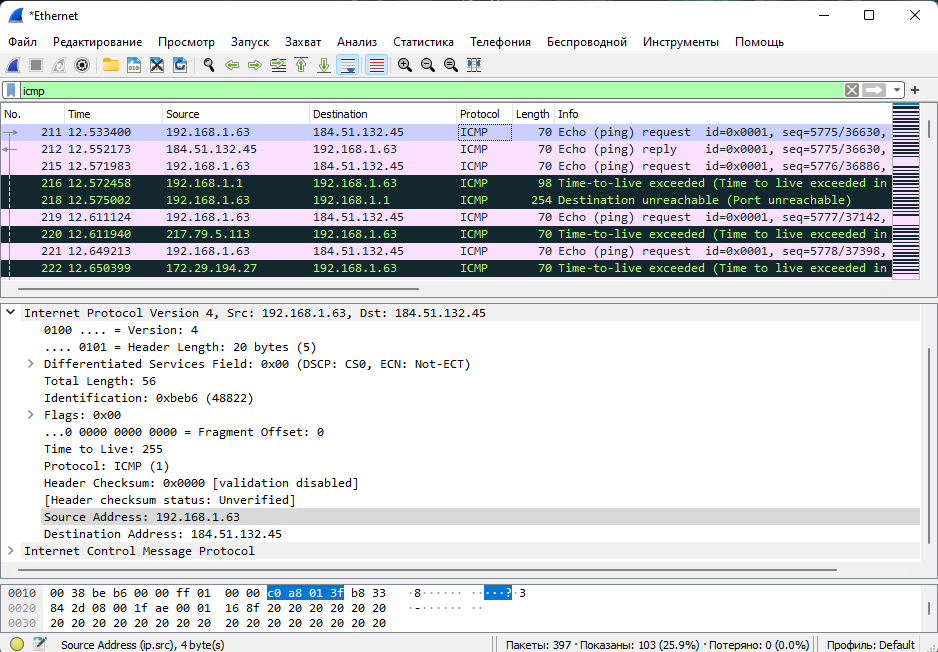
\includegraphics[width =\textwidth]{screenshots/1.png}}
\label{fig:image}
\end{center}
1) Source Address: 192.168.1.63

2) Protocol: ICMP (1)

3) Total Length: 56

.... 0101 = Header Length: 20 bytes (5)

Полезная нагрузка тогда 56 - 20 = 36

\begin{center}
\center{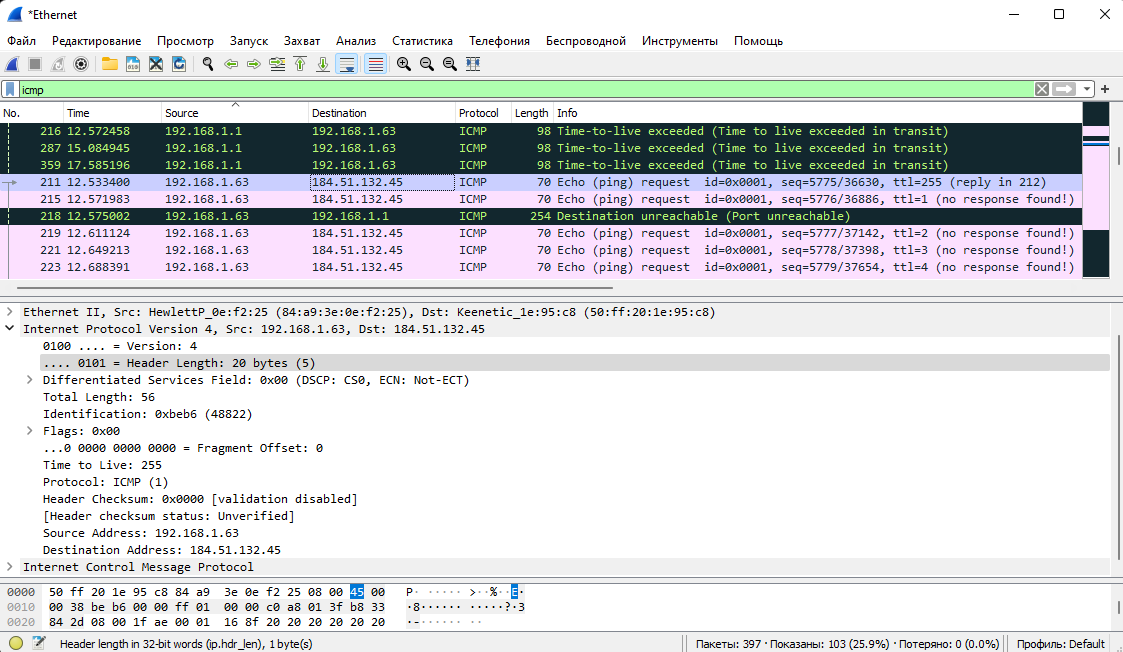
\includegraphics[width =\textwidth]{screenshots/2.png}}
\label{fig:image}
\end{center}

\begin{center}
\center{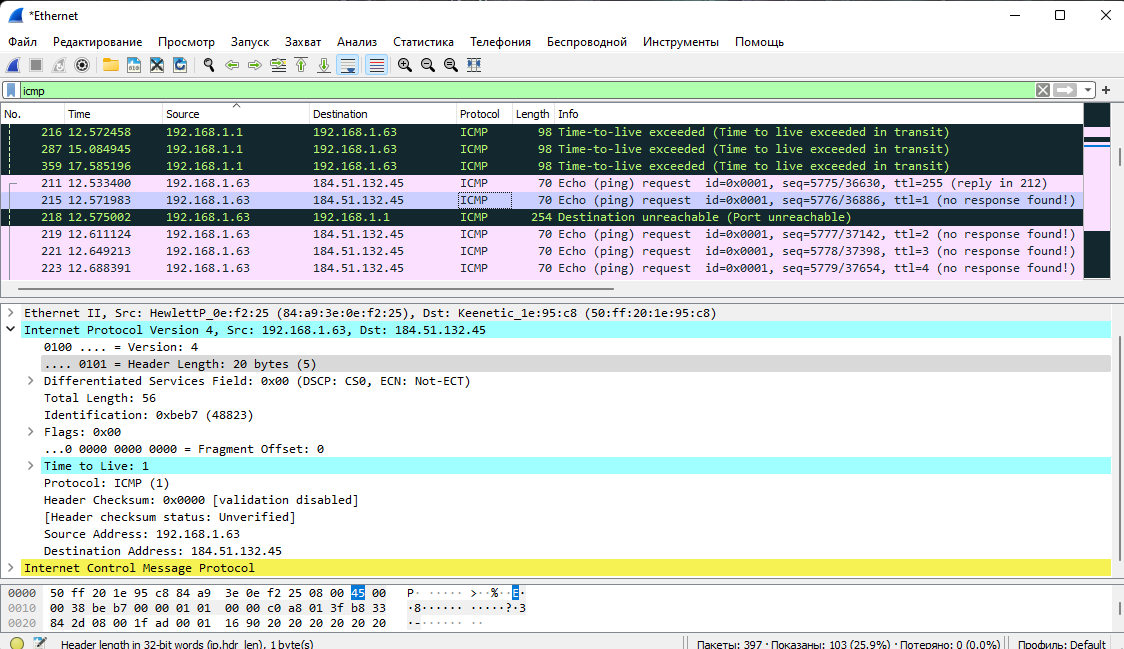
\includegraphics[width =\textwidth]{screenshots/3.png}}
\label{fig:image}
\end{center}
4) a)  TTL, Identification

b) Version, Length, Protocol, Checksum. TTL, Identification должны менятся (возможно еще Checksum, но везде 0x0000), остальные нет

c) Увеличивается на 1

5) Identification: 0xbeb6 (48822), Time to Live: 255

6) Нет, меняются

\begin{center}
\center{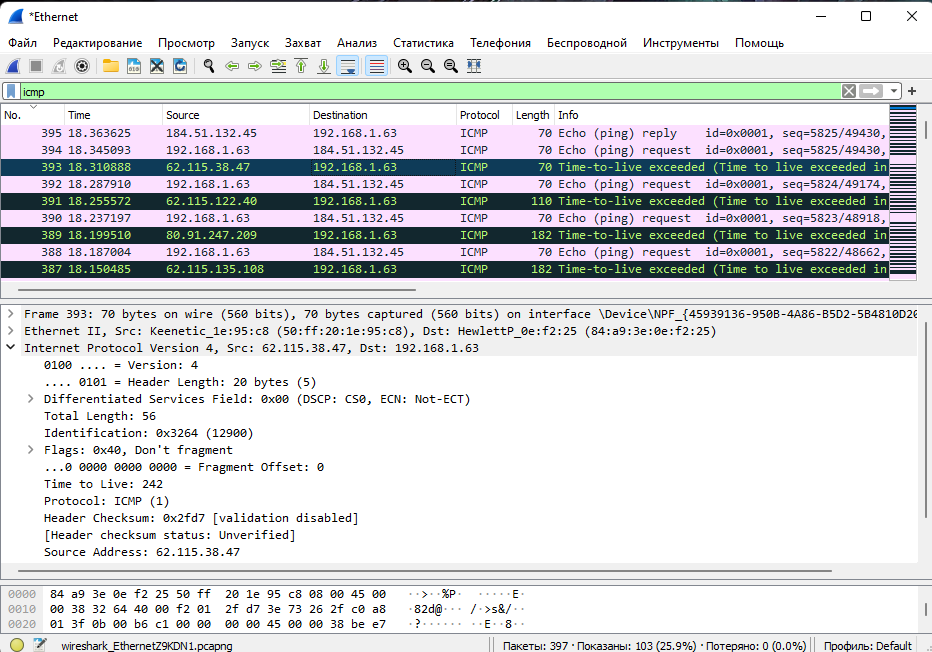
\includegraphics[width =\textwidth]{screenshots/4.png}}
\label{fig:image}
\end{center}
7) Identification: 0x3264 (12900), Time to Live: 242

\begin{center}
\center{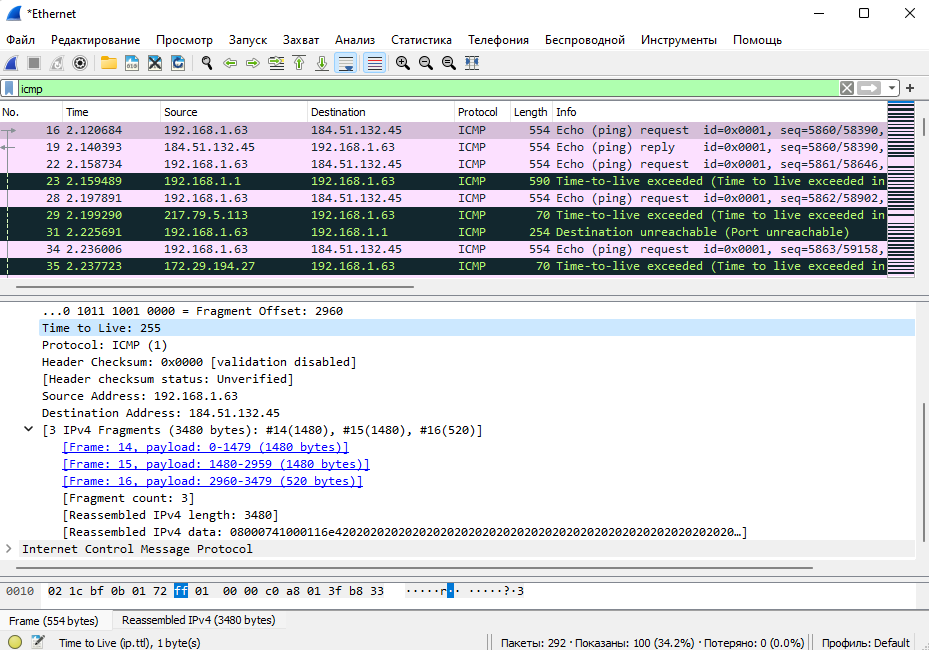
\includegraphics[width =\textwidth]{screenshots/5.png}}
\label{fig:image}
\end{center}
8) a) Да, [Fragment count: 3]

\begin{center}
\center{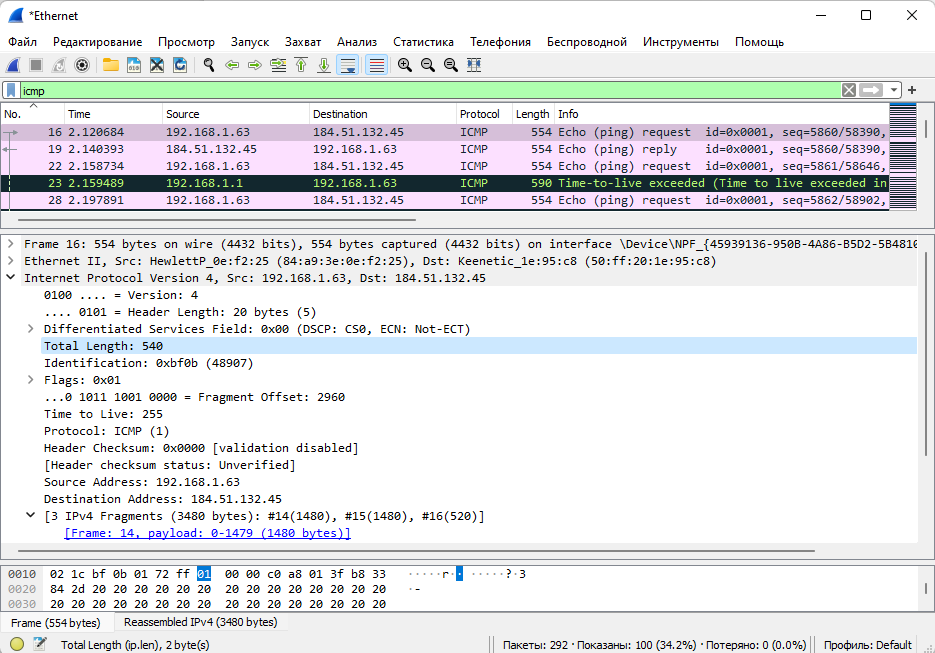
\includegraphics[width =\textwidth]{screenshots/6.png}}
\label{fig:image}
\end{center}
b) По сравнению с прошлым поменялись Length, Flags, Fragment Offset
\end{document}








































